\documentclass[11pt, a4paper, twoside, onecolumn]{book}
%\columnsep +30pt
\usepackage[margin=70pt]{geometry}
\usepackage{graphicx}
\usepackage{verbatim} 
\usepackage{wrapfig}
\usepackage[font={it}]{caption}
\usepackage{pgf-pie}
\usepackage{tabu}
\usepackage{url}

\usepackage[toc,page]{appendix}

\usepackage[cc]{titlepic}

%syntax highlighting
\usepackage{listings}
\lstset{language=C,
    numberstyle=\footnotesize,
    basicstyle=\ttfamily\footnotesize,
    numbers=left,
    stepnumber=1,
    frame=shadowbox,
    breaklines=true
}

% Pretty format chained footnotes with a comma.
\usepackage[multiple]{footmisc}

% Additional padding after the prefixed digit:
\let\oldfootnote\footnote
\renewcommand\footnote[1]{%
\oldfootnote{\hspace{2mm}#1}}

% Convenient shorthand functions:
\DeclareGraphicsExtensions{.png, .jpg}
\graphicspath{ {./images/} }

% Add references to table of contents:
\usepackage[nottoc]{tocbibind}

% Two column images:
\usepackage{subcaption}

% Clickable table of contents, hiding the colors.
\usepackage{hyperref}
\hypersetup{
    colorlinks,
    citecolor=black,
    filecolor=black,
    linkcolor=black,
    urlcolor=black
}
\hypersetup{pageanchor=false}


% Fix random page number alignment.
\usepackage{scrpage2}
\ifoot[]{}
\cfoot[]{}
\ofoot[\pagemark]{\pagemark}
\pagestyle{scrplain}

\title{
Some title
\\ \small \textit{Sub titles are cool too}
}


\author{ Gerard J. Meier \\ \small Kindergarten \\ \small \textit{gerjo.meier@hva.nl}}

\date{June 12, 2013}

\titlepic{\includegraphics[width=200px]{cover}}


\begin{document}
\maketitle

\section*{Abstract}

\tableofcontents

\chapter{Introduction}

% Just an image:
\begin{figure}[h]
\centering
\includegraphics[width=0.45\textwidth]{rotation}
\caption{The normal of each edge and its vertices are extended to run through the center-of-mass. Note that edge 'e' does not intersect with its normal, consequently it can be merged with edge 'a'.}
\label{fig:rotation}
\end{figure}

% Drawing polygons:
\begin{figure}[h]
    \centering
    \begin{subfigure}{.25\textwidth}
        \centering
        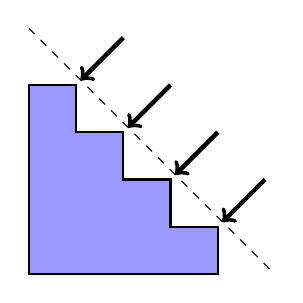
\begin{tikzpicture}[scale=0.6]
            
    \filldraw[thick,fill=blue,fill opacity=0.4] (0,0) -- (0,4) -- (1,4) -- (1,3) -- (2,3) -- (2,2) -- (3,2) -- (3,1) -- (4,1) -- (4,0) -- (0,0) -- cycle; 
            
            %fence
            \draw[dashed] (0,5.2) -- (5.2,0);

            %forces
            \draw[<-,ultra thick] (1.1,4.1) -- (2,5);
            \draw[<-,ultra thick] (2.1,3.1) -- (3,4);
            \draw[<-,ultra thick] (3.1,2.1) -- (4,3);
            \draw[<-,ultra thick] (4.1,1.1) -- (5,2);
        \end{tikzpicture}
        \caption{Concave polygon.}
    \end{subfigure}%
    \begin{subfigure}{.25\textwidth}
        \centering
        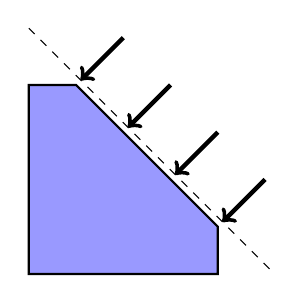
\begin{tikzpicture}[scale=0.6]
            
            % Concave polygon:
            
            \filldraw[thick,fill=blue,fill opacity=0.4] (0,0) -- (0,4) -- (1,4) -- (4,1) -- (4,0) -- (0, 0) -- cycle;

            %fence
            \draw[dashed] (0,5.2) -- (5.2,0);

            %forces
            \draw[<-,ultra thick] (1.1,4.1) -- (2,5);
            \draw[<-,ultra thick] (2.1,3.1) -- (3,4);
            \draw[<-,ultra thick] (3.1,2.1) -- (4,3);
            \draw[<-,ultra thick] (4.1,1.1) -- (5,2);
        \end{tikzpicture}
        \caption{Convex hull.}
    \end{subfigure}%
    
    \caption{Pushing forces act on the concave hull of any polygon. The dashed line represents a fence or lever as it comes in contact with a part.}
    \label{fig:hull}
\end{figure}


% Multiple columns, each with an image.
% Use \begin{figure*}[t] for a two column document.
\begin{figure}[h]
    \centering
    \begin{subfigure}{.33\textwidth}
        \centering
        
        \includegraphics[width=1\textwidth]{pfn1}
        
        \caption{Push function.}
    \end{subfigure}%
    \begin{subfigure}{.33\textwidth}
        \centering
        
        \includegraphics[width=1\textwidth]{pfn2}
        
        \caption{Push function.}
    \end{subfigure}%
    \begin{subfigure}{.33\textwidth}
        \centering
        
        \includegraphics[width=1\textwidth]{pfn3}
        
        \caption{Push function.}
    \end{subfigure}%
    
    \caption{Push functions visualized.}
    \label{fig:pushplots}
\end{figure*}

% A directed graph
\begin{figure}[h]
\centering
\begin{tikzpicture}[->,>=stealth',shorten >=1pt,auto,node distance=3cm,  thick,main node/.style={circle,fill=blue!20,draw}]  
    
\node[main node] (1) [label=$s_1$] {$\alpha_1$};
\node[main node] (2) [label=$s_2$, below left of=1] {$\alpha_1,\alpha_4$};
\node[main node] (3) [label=$s_3$, below right of=1] {$\alpha_1,\alpha_3$};
\node[main node] (4) [label=$s_4$, below left of=2] {$\alpha_1,\alpha_2,\alpha_3,\alpha_4$};
\node[main node] (5) [label=$s_5$, below left of=3] {$\alpha_2,\alpha_3$};  
\node[main node] (6) [label=below:$s_6$, below of=2] {$\alpha_2$};

\path[every node/.style={font=\sffamily\small}]    
(2) edge node[left] [] {} (1)
(3) edge node[right] [] {} (1)

(4) edge node[right] [] {} (2)
(5) edge node[right] [] {} (3)

(6) edge node[right] [] {} (2)
(6) edge node[right] [] {} (1)
(6) edge node[right] [] {} (5);



\end{tikzpicture}
\caption{An excerpt of a contrived graph of a fictional part with 4 possible equilibria. Each edge should be interpreted as "a fence exists such that". We observe that through 2 fences we can rotate this part to align with $\alpha_0$.}
\label{fig:exponential}
\end{figure}

\bibliographystyle{plain}

%nb: name your file refs.bib
\bibliography{refs}

\begin{comment}
This is a comment!
\end{comment}
\end{document}
